\documentclass[tikz,border=1pt]{standalone}
\usepackage{newtxtext,newtxmath}
\usetikzlibrary{arrows.meta,positioning,calc,decorations.pathmorphing}

\tikzset{
  >=Latex,
  line/.style={line width=0.8pt},
  % ラベルは白背景で塗って、線と重なっても可読に
  note/.style={font=\footnotesize,fill=white,inner sep=1pt,rounded corners=2pt},
  % Fig.2 のドロップ用
  dot/.style={draw,circle,fill=white,inner sep=0pt,minimum size=3.0mm,line width=0.8pt},
  smalldot/.style={dot,minimum size=2.6mm}
}

\begin{document}
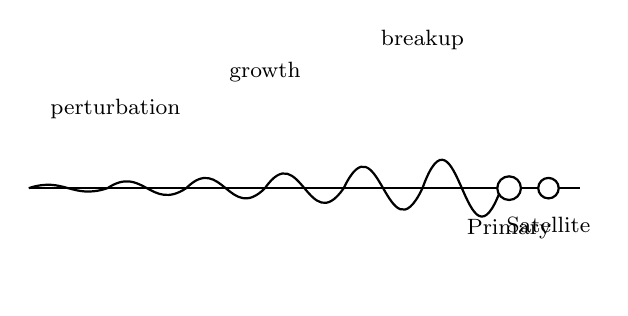
\begin{tikzpicture}[x=1.0cm,y=1.0cm]
  % --- jet axis
  \draw[line] (0,0) -- (7,0);

  % --- growing sinusoid-ish disturbance (段々振幅増加)
  \foreach \x/\a in {0/0.15,1/0.30,2/0.45,3/0.65,4/0.95,5/1.25}{
    \draw[line] (\x,0) .. controls +(.45,\a) and +(-.45,-\a) .. (\x+1,0);
  }

  % --- labels (白背景で上側に配置して重なり回避)
  \node[note,above=4pt] at (1.1,0.7) {perturbation};
  \node[note,above=6pt] at (3.0,1.1) {growth};
  \node[note,above=6pt] at (5.0,1.5) {breakup};

  % --- main & satellite drops
  \node[dot]      (main) at (6.10,0) {};
  \node[smalldot] (sat)  at (6.60,0) {};

  % --- captions (下側に少し余白をとって配置)
  \node[below=3pt of main, font=\footnotesize] {Primary};
  \node[below=3pt of sat,  font=\footnotesize] {Satellite};
\end{tikzpicture}
\end{document}
